\documentclass[a4paper,12pt]{article}
\usepackage[utf8]{inputenc}
\usepackage{polski, indentfirst}
\usepackage{amsmath}
\usepackage{csvsimple}

\usepackage{graphicx, float}

\title{Badanie wzmacniacza OE}
\date{15 października 2018}
\author{Filip Orłowski Paweł Nogaj Janusz Pajor}

\begin{document}

\maketitle
\newpage
\section{Wzmacniacz w konfiguracji OE}
Podstawowym elementem wzmacniacza jest tranzystor w~tym przypadku
bipolarny. Podaną konfigurację można zobaczyć na rysunku \ref{fig:oe}

\begin{figure}[H]
    \centering
    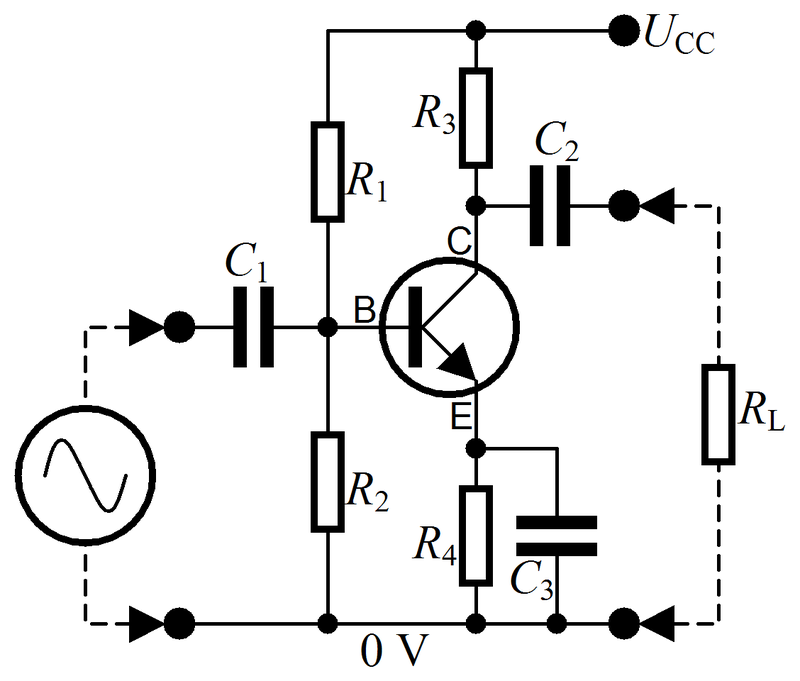
\includegraphics[width=10cm]{OE.png}
    \caption{Wzmacniacz OE}
    \label{fig:oe}
\end{figure}

\subsection{Rola poszczególnych elementów}
\begin{itemize}
    \item $C_1$ tworzy z theveniowską rezystanją zastępczą 
    dzielnika i $r_e $filtr górnoprzepustowy 
        \begin{equation*}
            f_c = \frac{1}{2\pi RC}
        \end{equation*}
    \item $C_2$ tworzy z rezystanją obciążenia $R_L$ filtr górnoprzepustowy
    \item $R_1$ i $R_2$ to dzielnik napięcia polaryzujący bazę tranzystora. Zwykle tak aby 
        \begin{equation*}
            U_{wy} = U_C = 0,5U_{cc}
        \end{equation*}
    \item $R_3$ wpływający bezpośrednio na wzmocnienie układu 
    \item $R_4$ rezystor emiterowy tzw. rezystor ujemnego sprzężenia zwrotnego;
        stabilizuje punkt pracy wzmacniacza

    \item $C_3$ dla składowej zmiennej zwiera $R_4$ tym samym zwiększając wzmocnienie układu
\end{itemize}

\subsection{Wzmocnienia układu}
Wzmocnienie napięciowe podawane jako iloraz napięcia wyjściowego do wejściowego:
\begin{gather*}
        G = \frac{U_{wy}}{U_{we}} [V/V] \\
        G = 20\log(\frac{U_{wy}}{U_{we}} ) [dB]
\end{gather*}
Wzmocnienie prądowe podawane jako iloraz prądu wyjściowego do wejściowego:
\begin{gather*}
    G = \frac{I_{wy}}{I_{we}} [V/V] \\
    G = 20\log(\frac{I_{wy}}{I_{we}} ) [dB]
\end{gather*}
Wzmocnienie mocy podawane jako iloraz mocy wyjściowej do wejściowej:
\begin{gather*}
    G = \frac{P_{wy}}{P_{we}} [V/V] \\
    G = 10\log(\frac{P_{wy}}{P_{we}} ) [dB]
\end{gather*}

\subsection{Pasmo przenoszenia}
Zakres częstotliwości, w którym tłumienie sygnału jest nie większe niż 3 dB
(spadek amplitudy o 3 dB w stosunku do amplitudy początkowej).
W paśmie przenoszenia amplituda osiąga wartość nie mniejszą niż 70,7\% swojej wartości maksymalnej.

\section{Układ pomiarowy}
Zadaniem ćwiczenia było wyznaczenie pasma przenoszenia przykładowego wzmacniacza OE.
Układ pomiarowy składał się z wzmacniacza OE, generatora przebiegów elektrycznych i oscyloskopu.
Za pomocą oscyloskopu i kalkulatora doknywaliśmy obliczania wzmocnienia napięciowego układu dla danych częstotliwości. 
Pomiary zostały zebrane w tabeli pomiarowej.
\subsection{Wykres}
W celu wyznaczenia pasma przenoszenia został wykonany prosty
program w Pythonie, który pobiera dane w formacie $*.csv$ rysuje wykres i podaje $f_g$ i $f_d$.
Pasmo przenoszenia jest widoczne na rysunku \ref{fig:wyk}.
\begin{figure}
    \centering
    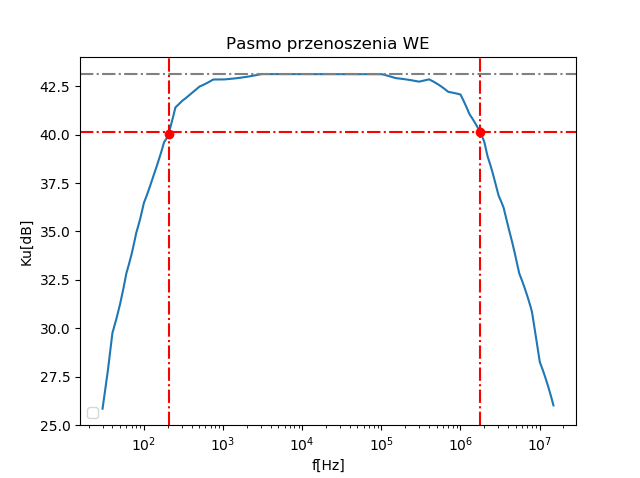
\includegraphics[width=15cm]{wykres.png}
    \caption{Pasmo przenoszenia $f_d = 205$Hz $f_g=1,78$MHz }
    \label{fig:wyk}
\end{figure}
\subsection{Oscyloskop cyfrowy}
Otwarcie zakładki pomiarowej jest możliwe po kliknięciu w przycisk
$Measure$, a następnie należy wybrać odpowiedni kanał lub kanały.
\newpage
\csvreader[tabular=|l|l|c|c|,
    table head=\hline & $f(Hz)$ & $G(V/V)$ & $G(dB)$\\\hline,
    late after line=\\\hline]%
{tr.csv}{f=\f,k=\k,db=\db}%
{\thecsvrow & \f & \k & \db}%

\end{document}
